\chapter{Radiation in Bending Magnets}\label{bendrad}
The theorie developed in \cite{Sands} will be first rewrited in order to clarify all terms used, making the proceeding generalization straight forward.
\section{Theoretical approximation}\label{radtheo}
Assuming a lattice that can be described by transport matrices in the form written in the Eq. (\ref{eq-matrix}), radiation effects can be calculated by the model in  \cite{Sands}.
\begin{equation}
\begin{pmatrix}
x_2\\
x'_2\\
\delta
\end{pmatrix}
=
\begin{pmatrix}
 C(s_1,s_2) & S(s_1,s_2)& R_{16}(s_1,s_2)\\
 C'(s_1,s_2) & S'(s_1,s_2) & R_{26}(s_1,s_2)\\
 0 & 0 &1
\end{pmatrix}
\begin{pmatrix}
x_1\\
x'_1\\
\delta
\end{pmatrix}
\label{eq-matrix}
\end{equation}
Being $\Delta x_i = R_{16}(s_i,s_p) (-u)/E$, the deviation at the observation point $s_p$ due to the $i^{\text{th}}$ photon of energy $u$ radiated at some point $s_i$, and $E$ the beam energy.\par The first rhs term in Eq. (\ref{eq-sumphot}) is the sum over the $N$ photons radiated during the time $T$ for the particle to cross the magnet. $N(T)$ describes the probability distribution of photon emission. As we are interested only in the second order moment, the mean  $x_0=\langle\sum_{i=1}^{N(T)}\Delta x_i\rangle$ is subtracted from the sum, obtaining $\langle x\rangle=0$, $ \sigma_{bend}^2=\langle x^2\rangle$, being $x$ the horizontal transverse displacement from the reference orbit of a particle at the observation point.
\begin{equation}
\sum_{i=1}^{N(T)}\Delta x_i - x_0 = x\label{eq-sumphot}
\end{equation}
The photon emission follows a Poisson distribution as a consequence of the normalized radiation spectrum and photon number spectrum of synchrotron radiation used in \cite{Sands2} Section 5. For any Poisson-like distribution $\sigma_N^2 = \langle N\rangle$. The beam size contribution due to radiation has two components of variability: the spread of $\Delta x_i$ due to the energy emission $u$ and the number of times the emission process occurs $N$\footnote{Using statistics notation, $\sigma_x=V(x)$ and $\langle x\rangle=E(x)$, then, a process with two components of variability has a variance expressed as $V(x)=E(V(x|N))+V(E(x|N))$. The term $(x|N)$ denotes the evaluation of the $x$ variable for a given $N$}. Therefore, it is calculated as in Eq. (\ref{eq-bsize})
\begin{align}
\sigma^2_{bend} &= \langle x^2\rangle - \cancelto{0}{\langle x\rangle^2} = \langle x^2 \rangle\label{eq-bsize}\\
 &= \langle N\rangle \sigma^2_{\Delta x} + \langle \Delta x \rangle ^2 \sigma_N^2\\
 &= \langle N\rangle \langle (\Delta x)^2\rangle -\cancel{\langle N\rangle\langle\Delta x\rangle^2} + \cancel{\langle \Delta x \rangle^2\langle N \rangle}\\
 &=\langle N\rangle \langle (\Delta x)^2\rangle
\end{align}
Where the $i$ sub-index has been removed intentionally because the photon number emission is extracted from a continuous function of $u$ the photon energy and either $T$ or $s/c$, where $c$ is the speed of light.\par 
The rate of emission of photons is calculated as in Eq. (\ref{eq-nu}) where $K_{5/3}$ is the modified Bessel function, $u_c=\frac{3}{2}\frac{\hbar c \gamma^3}{\rho}$ called the critical energy which depends on the relativistic factor $\gamma$, the reduced Planck constant $\hbar$ and the particle trajectory curvature $\rho$, and $P_\gamma=\frac{2cr_emc^2}{3\rho^2}\gamma^4$ is the instantaneous radiated power where $r_e$ is the classical electron radius and $m$ is the electron mass.
\begin{equation}
n(u,s)=\frac{P_\gamma}{u_c^2}\left[\frac{9\sqrt{3}}{8\pi}\int_{u/u_c}^\infty K_{5/3}(\xi) d\xi\right]\label{eq-nu}
\end{equation}
Using $\Delta x(s) = (-u/E) R_{16}(s,s_p)$ the second moment is calculated by integration over the entire space and energies.
\begin{align}
 \sigma_{bend}^2&=\int_0^{T} \int_0^\infty [\Delta x(u,s)]^2 n(u,s)dudT\label{eqDeltaX}\\
 &=\frac{1}{c}\int_0^{s_p} \int_0^\infty \left[\frac{-u}{E}R_{16}(s,s_p)\right]^2 n(u,s)duds\\
\end{align}
Finally, 
\begin{equation}
\sigma^2_{bend}=C_2\int_0^{s_p} \frac{E^5}{\rho^3}R_{16}(s,s_p)^2 ds\label{eq-R16}
\end{equation}
where $C_2=\frac{55}{24\sqrt{3}}\frac{r_e\hbar c}{(mc^2)^6}=4.13\times10^{-11} \text{ m}^2\text{GeV}^{-5}$ is a constant coming from the emission rate integration already derived by Sands.\par
\section{Generalization when final dispersion is not zero}
It is common to have direct access to Twiss functions over the lattice, therefore, it is also convenient to use Eq. (\ref{eq-matrix}) to calculate $R_{16}$ from the off-momentum function $\eta$ and lattice parameters. Measuring from the reference orbit, the kick propagation from $s$ to $s_p$ can be written in terms of the general transport matrix, giving
\begin{align}
\Delta x(s)_{total}=\frac{-u}{E}\eta(s_p) &= \frac{-u}{E} \left[C(s,s_p)\eta(s) + S(s,s_p)\eta'(s) + R_{16}(s,s_p)\right]\\
\eta(s_p) &= \sqrt{\frac{\beta_{s_p}}{\beta_s}}\left[\eta_s\cos\Delta\phi_{s,s_p}+(\alpha_s\eta_s+\beta_s\eta'_s)\sin\Delta\phi_{s,s_p}\right] + R_{16}(s,s_p)\label{eq-disp}
\end{align}
where $\alpha, \beta$ and $\phi$ are the optics parameters and the subscripts indicate the evaluation point. The equations derived in \cite{Sands} assume $\alpha_{s_p}=0, \eta_{s_p}=0$ and $\eta'_{s_p}=0$, which are not valid during the lattice optimization process. From Eq. (\ref{eq-R16}) and (\ref{eq-disp}) is clear that the contribution to beam size due to radiation now can be calculated as:
\begin{equation}
 \sigma_{bend}^2=C_2 \int_0^{s_p} \frac{E^5_s}{\rho^3_s}\left\{\sqrt{\frac{\beta_{s_p}}{\beta_s}}\left[\eta_s\cos\Delta\phi_{s,s_p}+(\alpha_s\eta_s+\beta_s\eta'_s)\sin\Delta\phi_{s,s_p}\right]-\eta_{s_p}\right\}^2ds\label{eq-radbends}
\end{equation}
Eq. (\ref{eq-radbends}) was included in MapClass2 in order to be used during lattice design and optimization.\par

\section{One dipole}
A theoretical calculation has been derived for the case of one sector magnet ($\rho,L,\theta$) and a sector magnet plus a drift ($L_{drift}$). Beam energy loss is negligible compared with beam energy $E$.\par
For a sector magnet, $R_{16}= \rho(1-\cos\theta)$, the radiation effect is calculated as follows
\begin{align}
\sigma_{bend}^2 &= C_2 E^5\int_0^\theta \frac{1}{\rho^3}[\rho(1-\cos(\theta-\chi))]^2\rho d\chi\\
&= C_2E^5\left[\frac{1}{4}(6\theta-8\sin\theta+\sin(2\theta))\right]\label{eqNum}\\
&=C_2E^5\left(\frac{\theta^5}{20}-\frac{\theta^7}{168}+\frac{\theta^9}{2880}-\frac{17\theta^{11}}{1330560}+O(\theta^{13})\right)
\end{align} 
 In the case of a drift after the bending magnet and defining $j=\frac{L_{drift}}{\rho}=\frac{L_{drift}}{L}\theta$
\begin{align}
  \sigma_{bend}^2 =& C_2 \int_0^\theta E^5\left[1-\cos(\theta-\xi)+\frac{L_{drift}}{\rho}\sin(\theta-\xi)\right]^2 d\xi\\
 =& \frac{C_2}{4} E^5 \left[(1-j^2)\sin(2\theta)-8\sin\theta+4j(1-\cos\theta)^2+(6-2j^2)\theta\right]\label{eqNum2}\\
  =& C_2 E^5 \left[\frac{j^2\theta^3}{3}+\frac{j\theta^4}{4}-\frac{(4j^2-3)\theta^5}{60}- \frac{j\theta^6}{24} +\frac{(16j^2-15)\theta^7}{2520}+\frac{j\theta^8}{320}\right.\notag\\
    &-\frac{(64j^2-63)\theta^9}{181440}-\frac{17j\theta^{10}}{120960}+\frac{(256j^2-255)\theta^{11}}{19958400}+\frac{31j\theta^{12}}{7257600}\notag\\
    &\left.-\frac{(1024j^2-1023)\theta^{13}}{3113510400}+O(\theta^{14})\right]
\end{align}
Eqs. (\ref{eqNum}) and (\ref{eqNum2}) will be used to normalize the results from MAPCLASS2 and PLACET \cite{Placet} where some care should be taken due to numerical precision.\par
\section{MAPCLASS2 and PLACET results}
In PLACET 0.99.01 two different implementations of radiation exist: the first one will be called `default' and the second `six\_dim'. `Default' calculates radiation by segmenting the dipole in shorter pieces, what is called thin dipole approximation, while `six\_dim' does not make any sectioning of the dipole. Results from these implementations and from MAPCLASS2 can be seen in Fig. \ref{figSR}, normalized to the theoretical values in Eqs. (\ref{eqNum}) and (\ref{eqNum2}). The energy is 1500 GeV in all cases.\par
Calculation of radiation effect in PLACET was done by subtracting the squared beam size from two trackings with same input parameters except for radiation ON/OFF. As PLACET 0.99.01 does not give an uncertainty value, fitting was made once on the raw particle data with total agreement with the PLACET reported value, therefore, the error bars come from statistics assuming error of $1/\sqrt{M}$ with $M$ the number of tracked particles, 100000 particles in all cases.\par
All required Twiss functions were calculated using `ptc\_twiss' 5 dim in MAD-X \cite{MADX}. However, they have discrepancies for very low angles as it is shown in Fig. \ref{figSR}(a) and (b) showing abrupt changes close to $\theta=7.5\times10^{-6}$ rad. The validity of the model for such low angles is still under discussion.
\begin{figure}[htb]
\centering
  \hspace*{1.2cm}`Default' Synrad\hspace*{5.0cm}Flag `-six\_dim 1'\par
 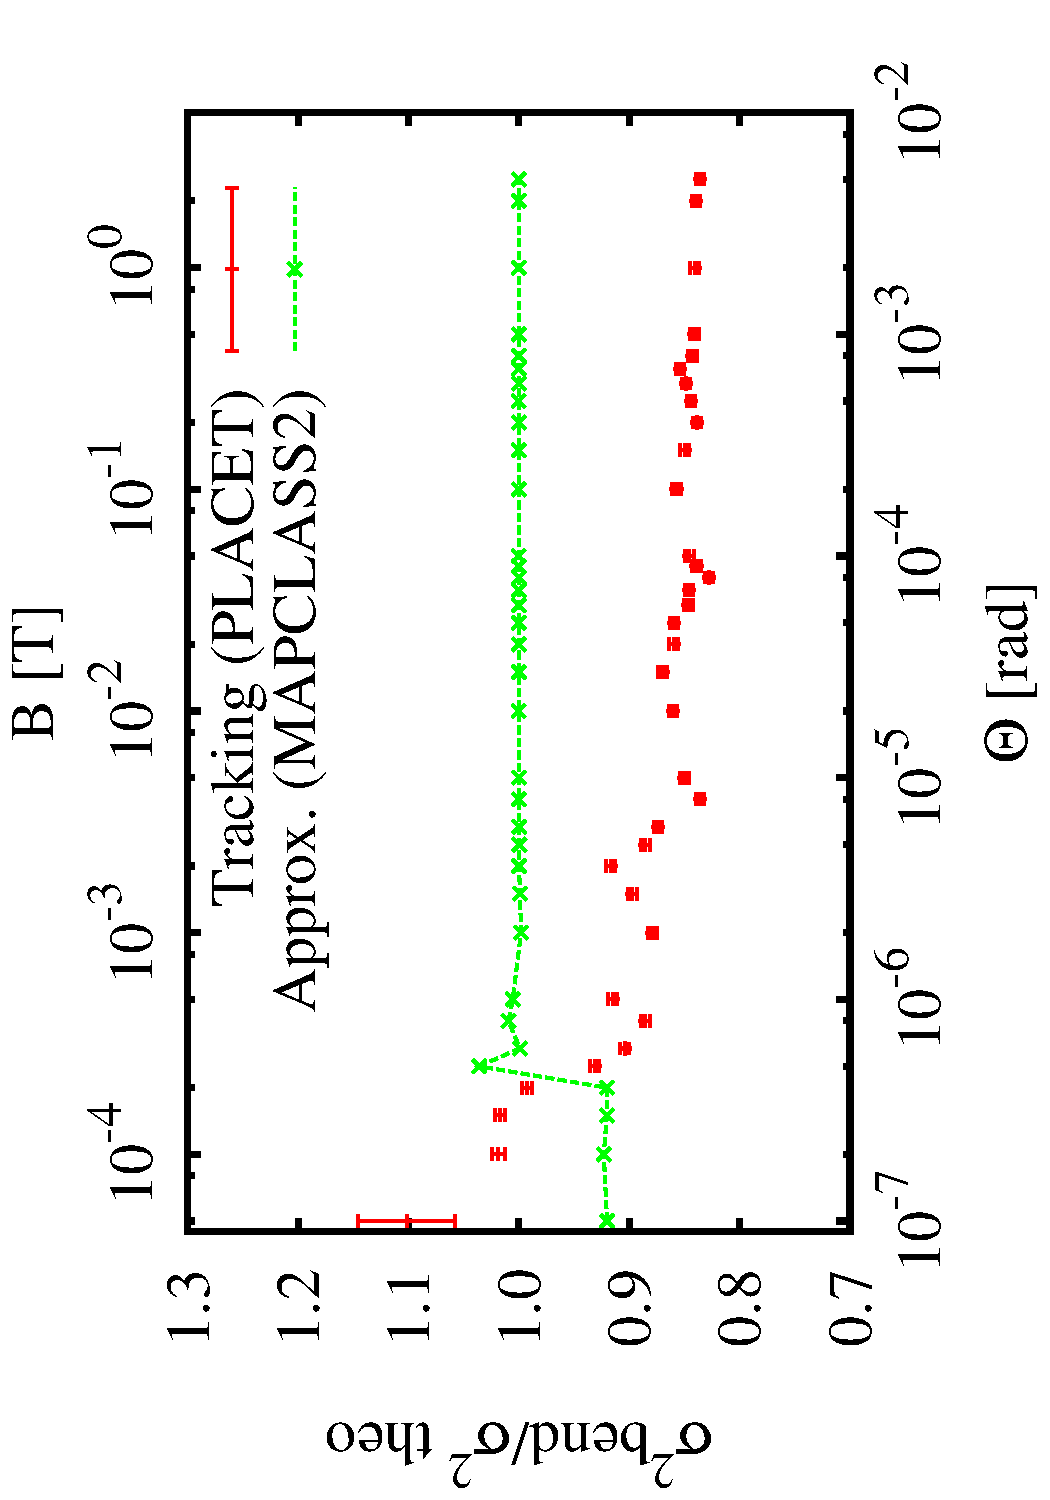
\includegraphics[scale=0.30,angle=-90]{sigma_angle.pdf}
  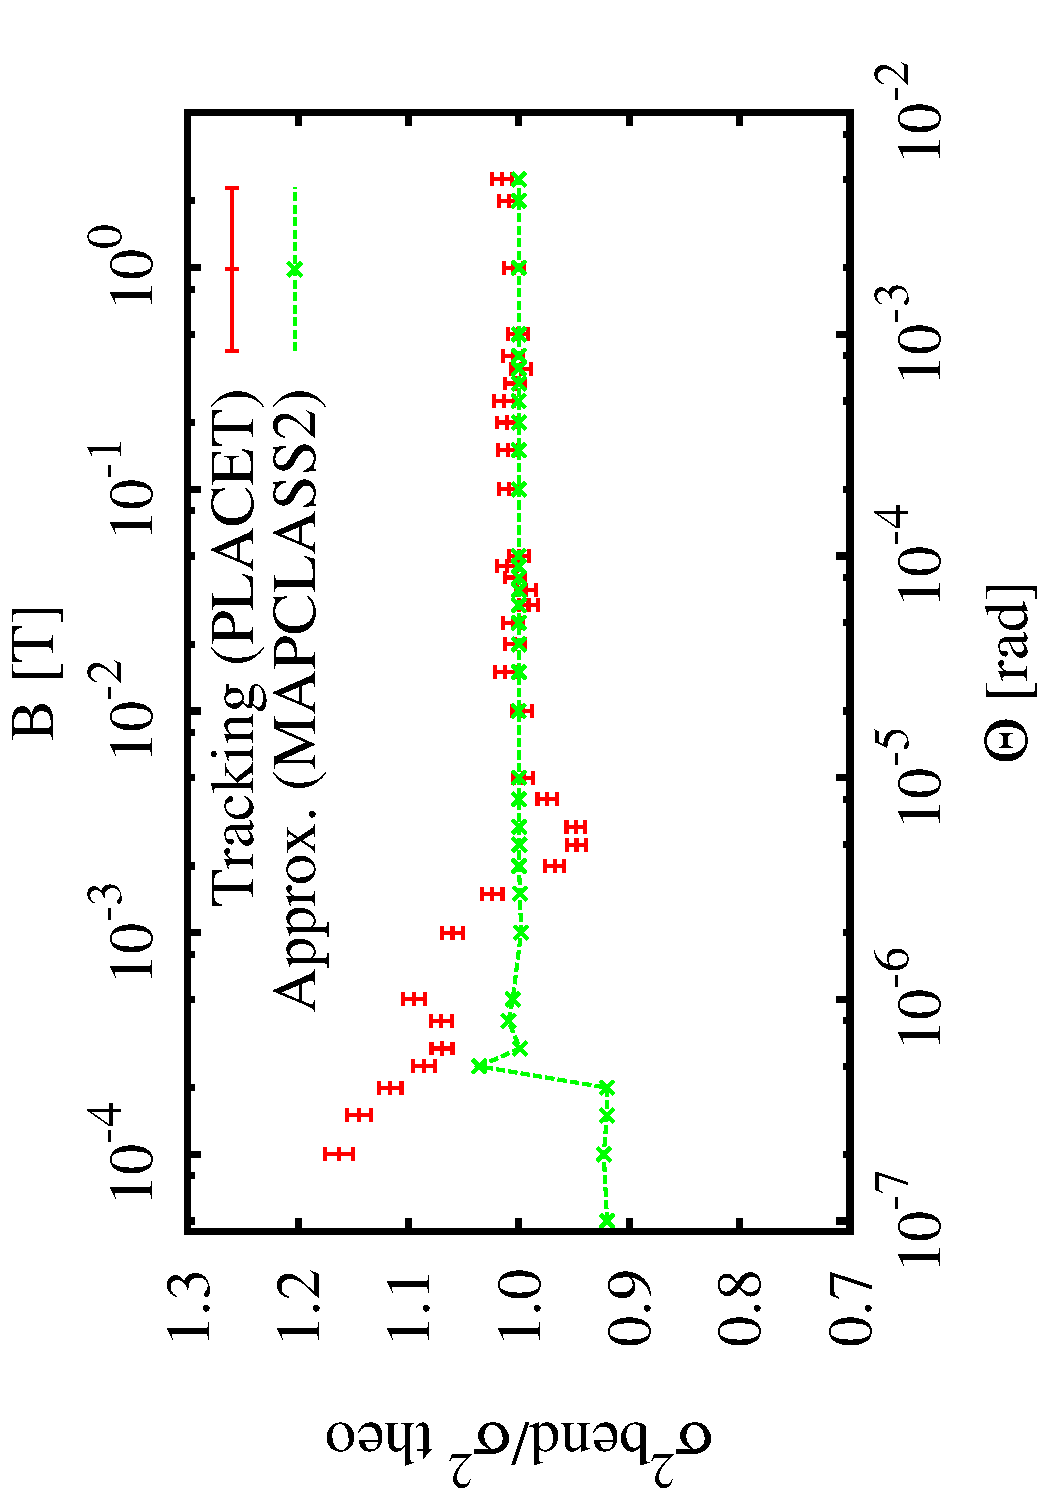
\includegraphics[scale=0.30,angle=-90]{sigma_angle_r06.pdf}\par
  \hspace*{1.0cm}(a)\hspace*{7.6cm}(b)\par
   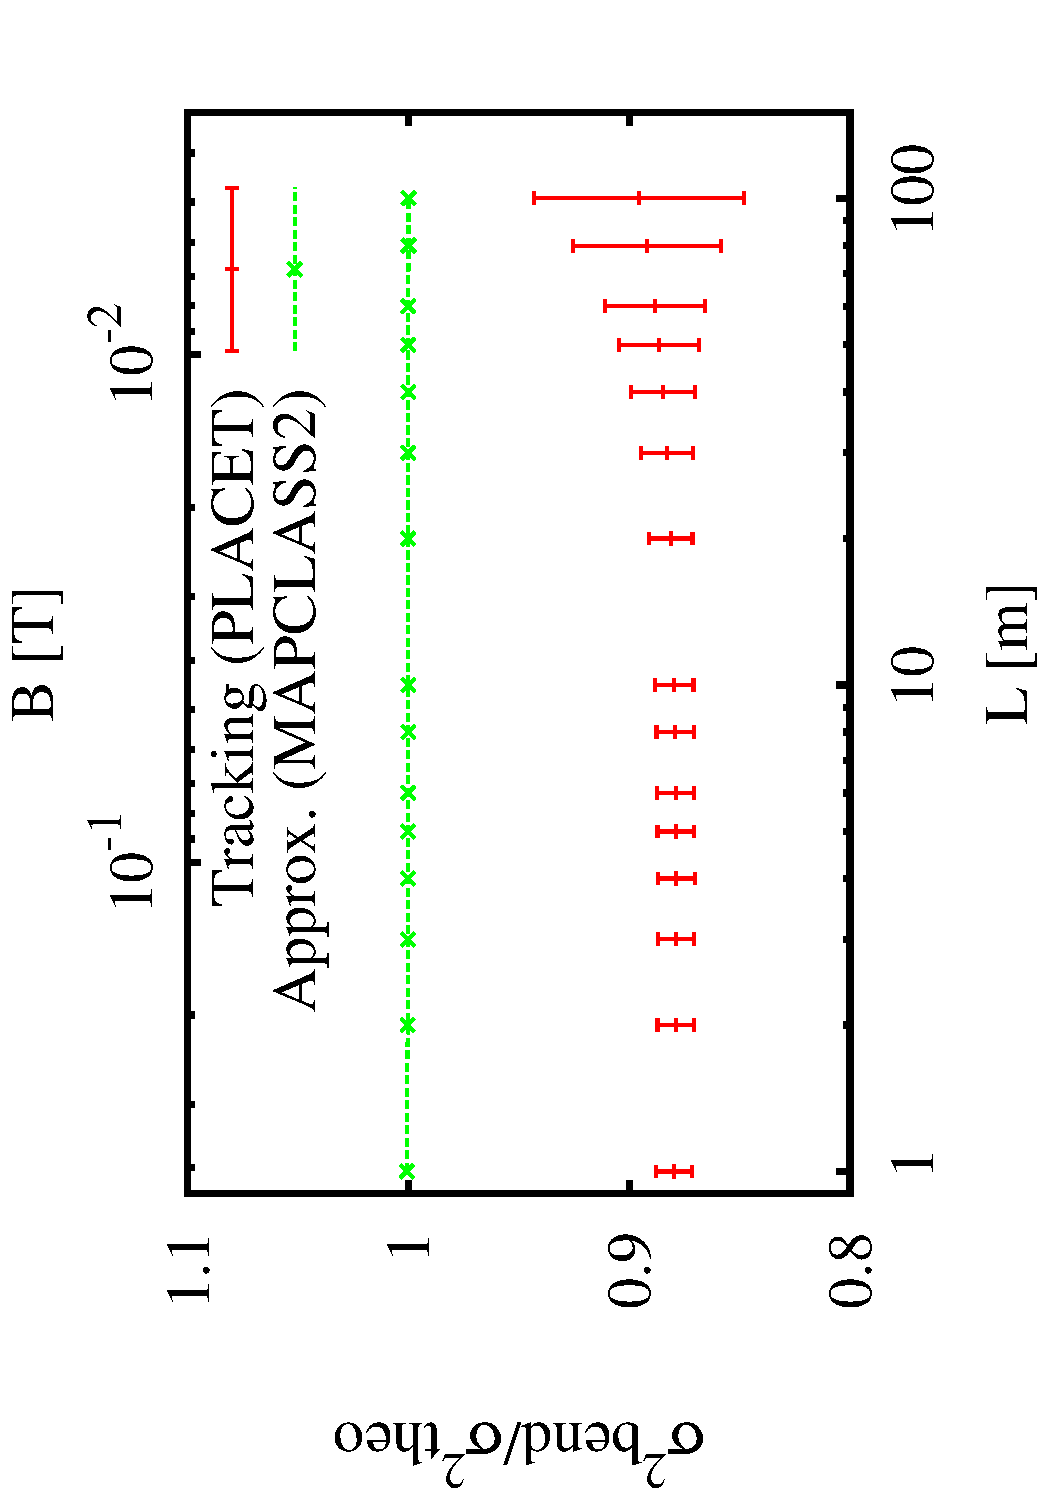
\includegraphics[scale=0.30,angle=-90]{sigma_Lbend.pdf}
  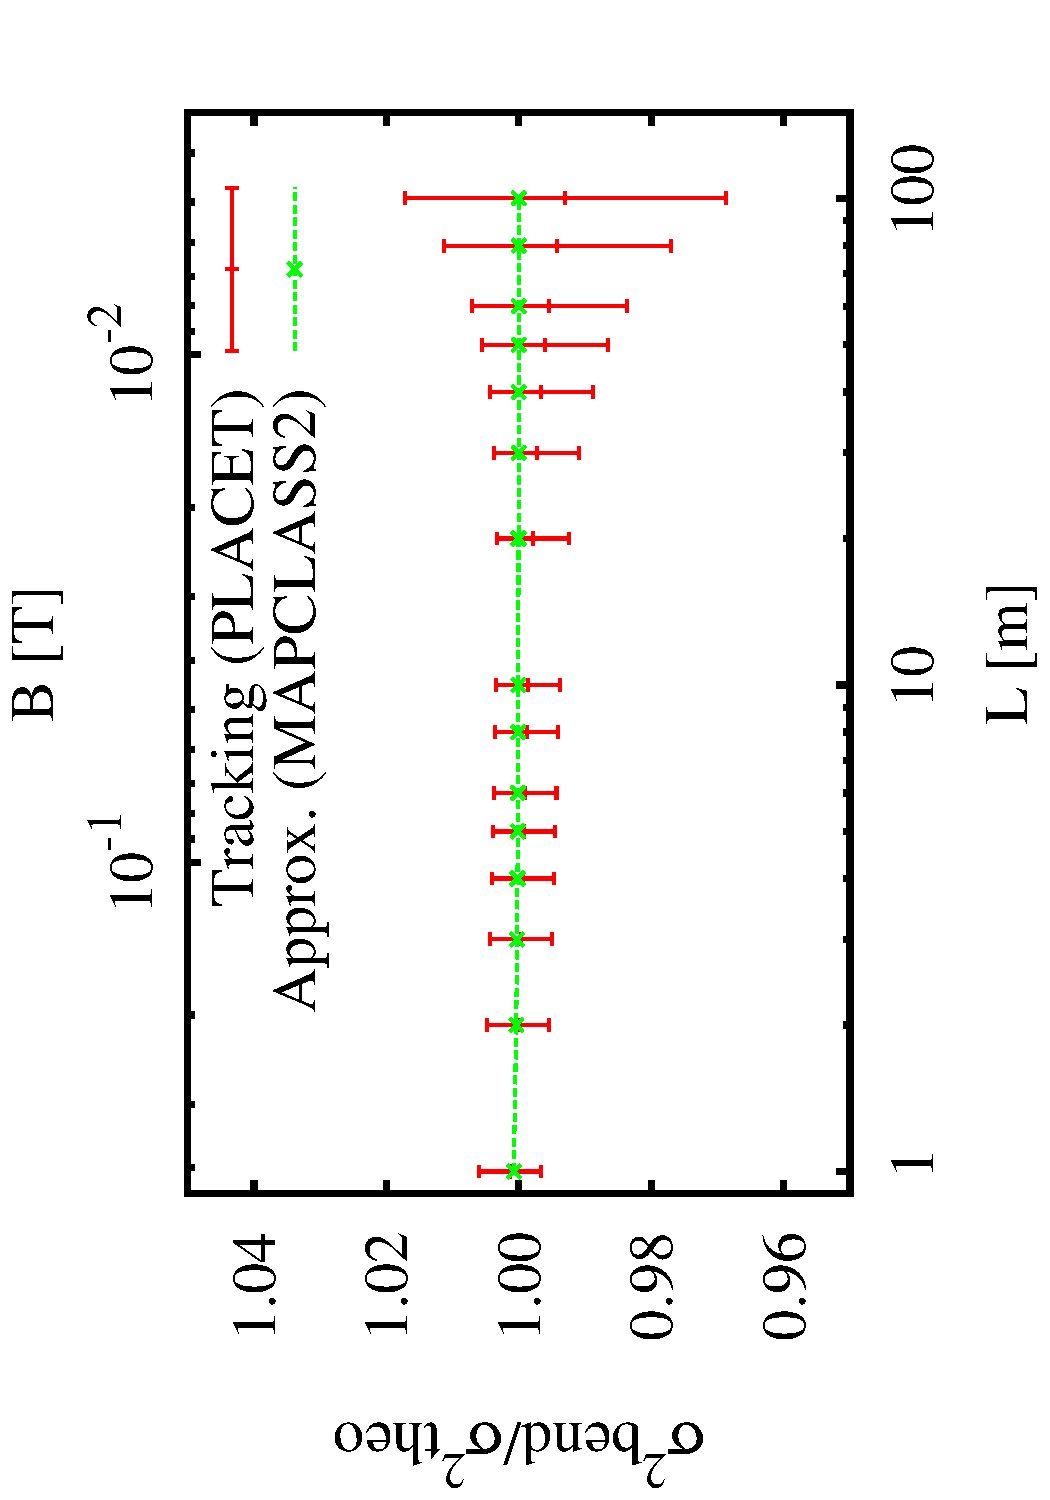
\includegraphics[scale=0.30,angle=-90]{sigma_Lbend_r6.pdf}\par
  \hspace*{1.0cm}(c)\hspace*{7.6cm}(d)\par
  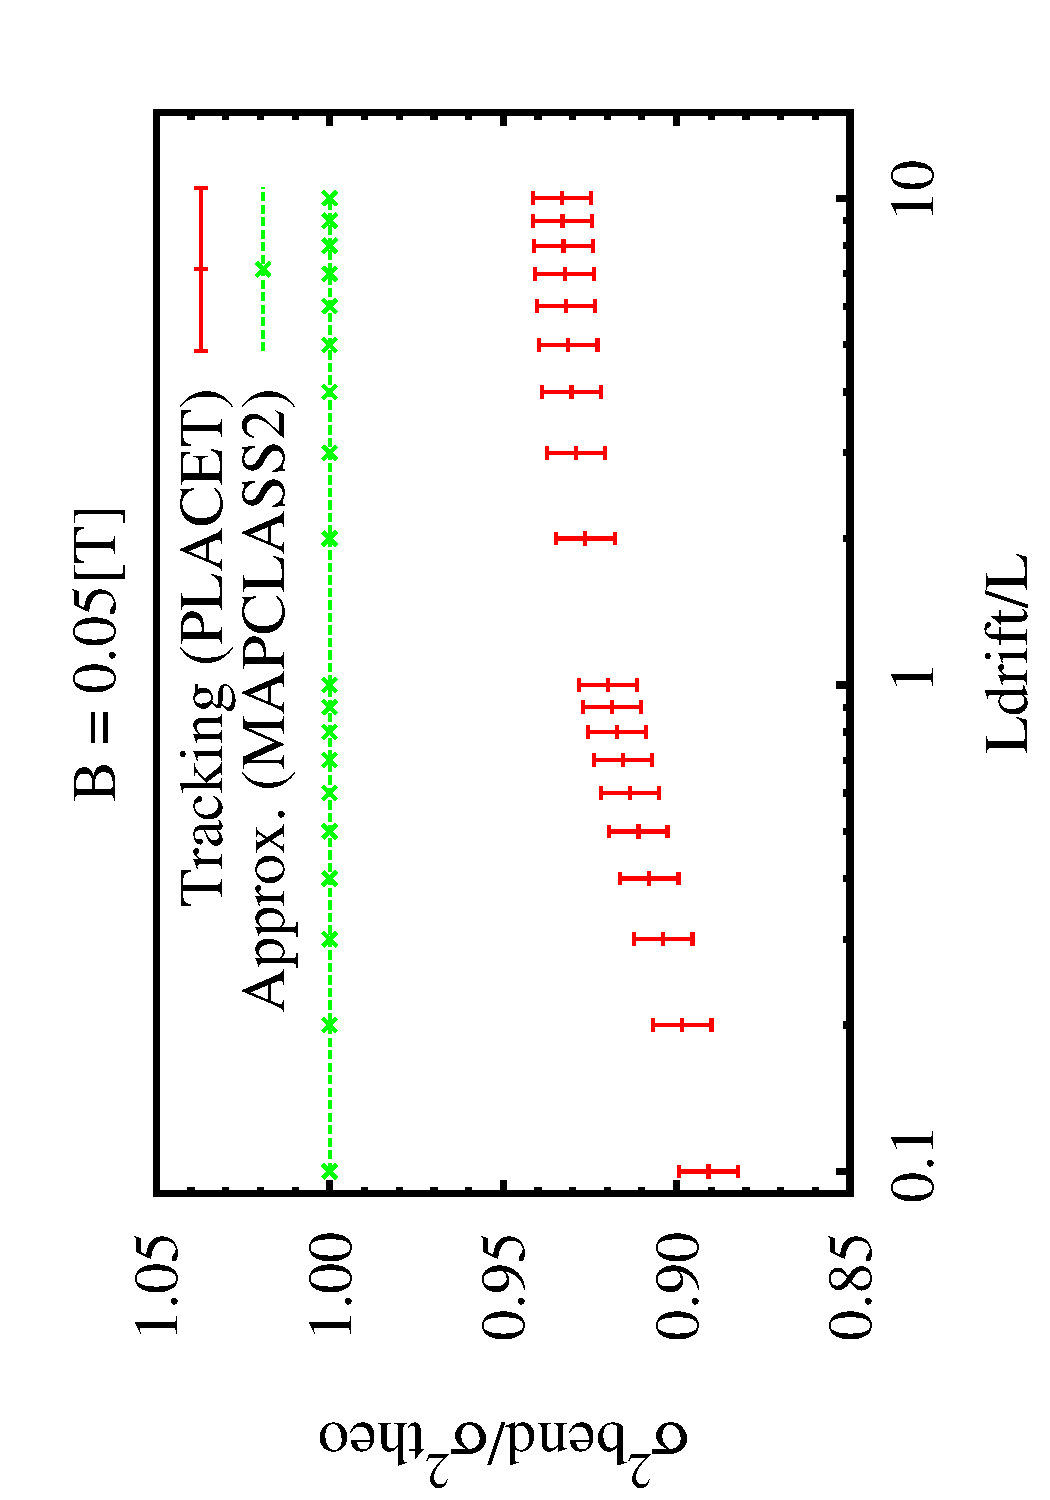
\includegraphics[scale=0.30,angle=-90]{sigma_Ldrift.pdf}
  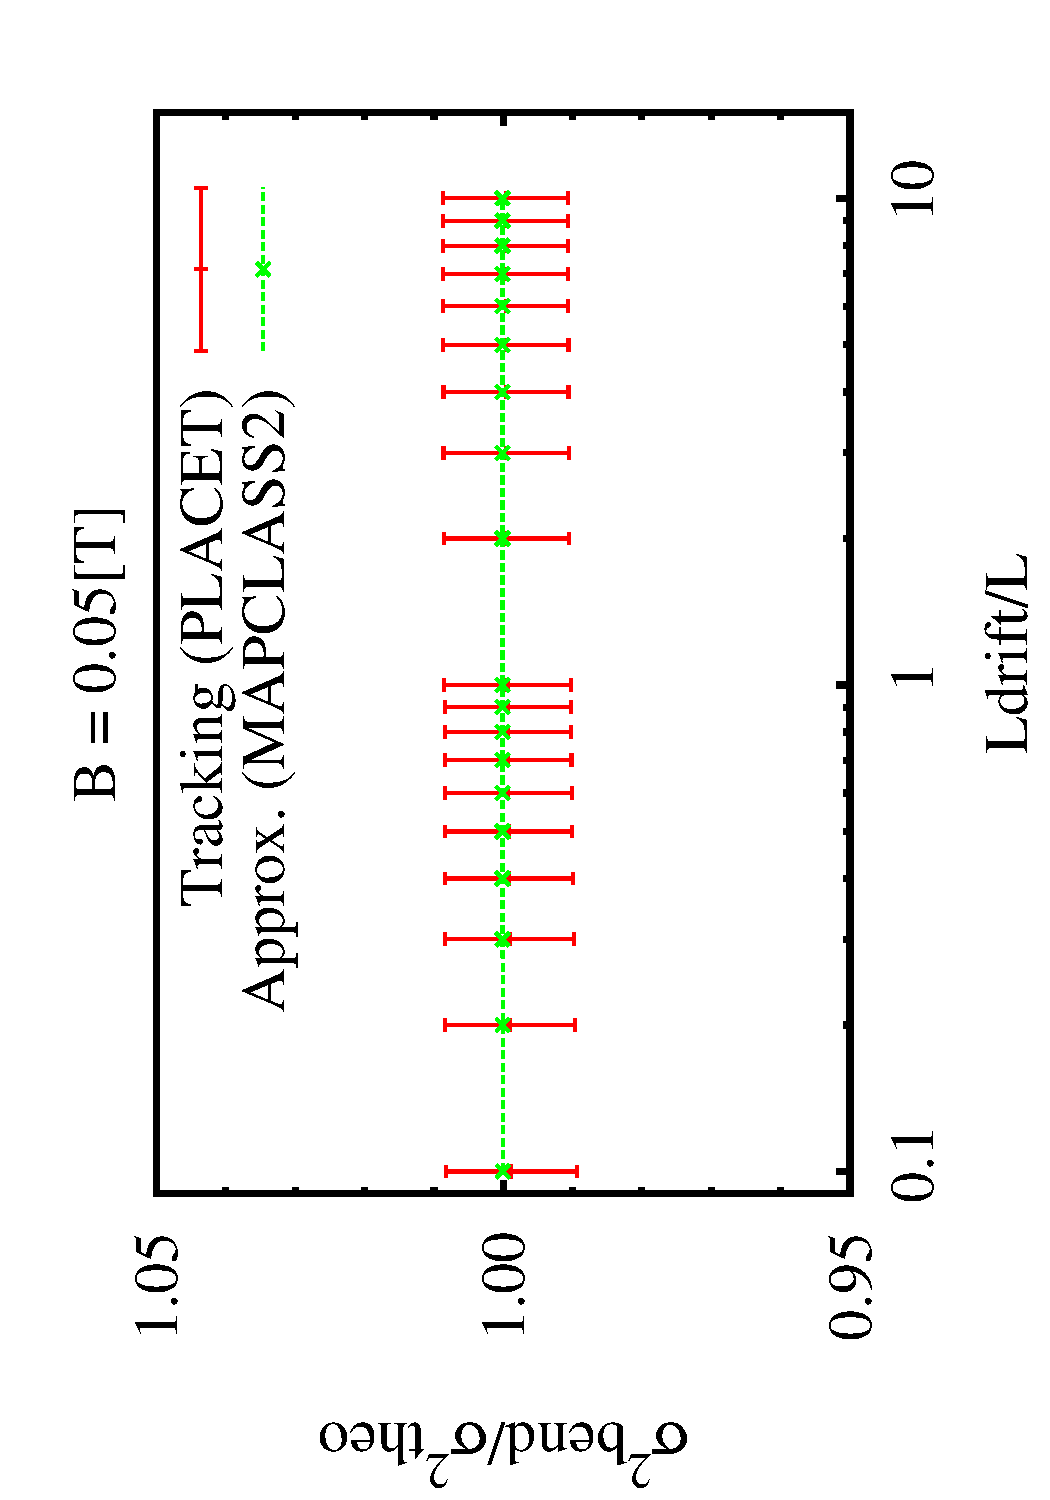
\includegraphics[scale=0.30,angle=-90]{sigma_Ldrift_r6.pdf}
  \hspace*{1.0cm}(e)\hspace*{7.6cm}(f)\par
\caption{Beam size increase due to radiation normalized to theoretical value assuming negligible energy loss. (Left) `Default' radiation option, (Right) `Six\_dim' option in PLACET 0.99.01. Plots (a) and (b) correspond to $L=10$ m for a dipole only. Plots (c) and (d) correspond to $\theta=10^{-4}$ rad for a dipole only. Plots (e) and (f) correspond to $L=10$ m and $\theta=10^{-4}$ rad while varying the drift length. Beam energy is 1500 GeV in all cases.}\label{figSR}
\end{figure}
\clearpage
\section{Validity for the FFS}
The radiation model presented is valid when the average number of photons radiated per particle $\langle N\rangle$ is enough to characterize the overall effect in position by its second moment, where $\langle N\rangle  = C_1E\theta$ with $C_1=20.61\text{ GeV}^{-1}$.\par
The CLIC FFS design is composed by magnets with bending angles shown in Table \ref{T-nphotons_3TeV} for 3 TeV and Table \ref{T-nphotons_500GeV} for 500 GeV. Although the average value of photons emitted per magnet is low, these are grouped in long sections with common bending angle. The third column indicates the quantity of magnets used in each of those sections.
\begin{table}[ht]
\begin{minipage}[b]{0.45\linewidth}\centering
\begin{tabular}{c|c|c}\hline\hline
 $|\theta|$ & $\langle N \rangle$&Qty.\\
 ($\mu$rad)&&\\\hline
 $\;\;$1.1& 0.07 &70 \\
 $\;\;$3.9& 0.24 &20 \\
 17.2& 1.06 &10\\\hline
\end{tabular}\caption{Bending angles in CLIC 3 TeV.}\label{T-nphotons_3TeV}
\end{minipage}
\hspace{0.5cm}
\begin{minipage}[b]{0.45\linewidth}
\centering
\begin{tabular}{c|c|c}\hline\hline
 $|\theta|$& $\langle N \rangle$&Qty.\\
 ($\mu$rad)&&\\\hline
 $\;\;\;\;$8.3& 0.08&70\\
 $\;\;$27.5& 0.28 &20\\
 135.0& 1.39 &10\\\hline
\end{tabular}\caption{Bending angles in CLIC 500 GeV.}\label{T-nphotons_500GeV}
\end{minipage}
\end{table}

\section{Cases where the model fails}
Particle tracking gave dissimilar results when compared with theory for magnetic fields lower than $5\times 10^{-3}$ T as is shown in Fig. \ref{figSR}(b). When calculating the average number of photons emitted by particle $\langle N\rangle$, it seems that there is a connexion between the one photon threshold and the dissimilarity, see Fig. \ref{figPhotons} where the magnetic field was fixed at $5 \times 10^{-3}$ T. %Although, cases where less than one photon is emitted per particle on average are supposed to be negligible, it might become significant due to the amount of particles.\par
Changes in the model might need to be revisited on this magnetic field range.
\begin{figure}[htb]
\centering
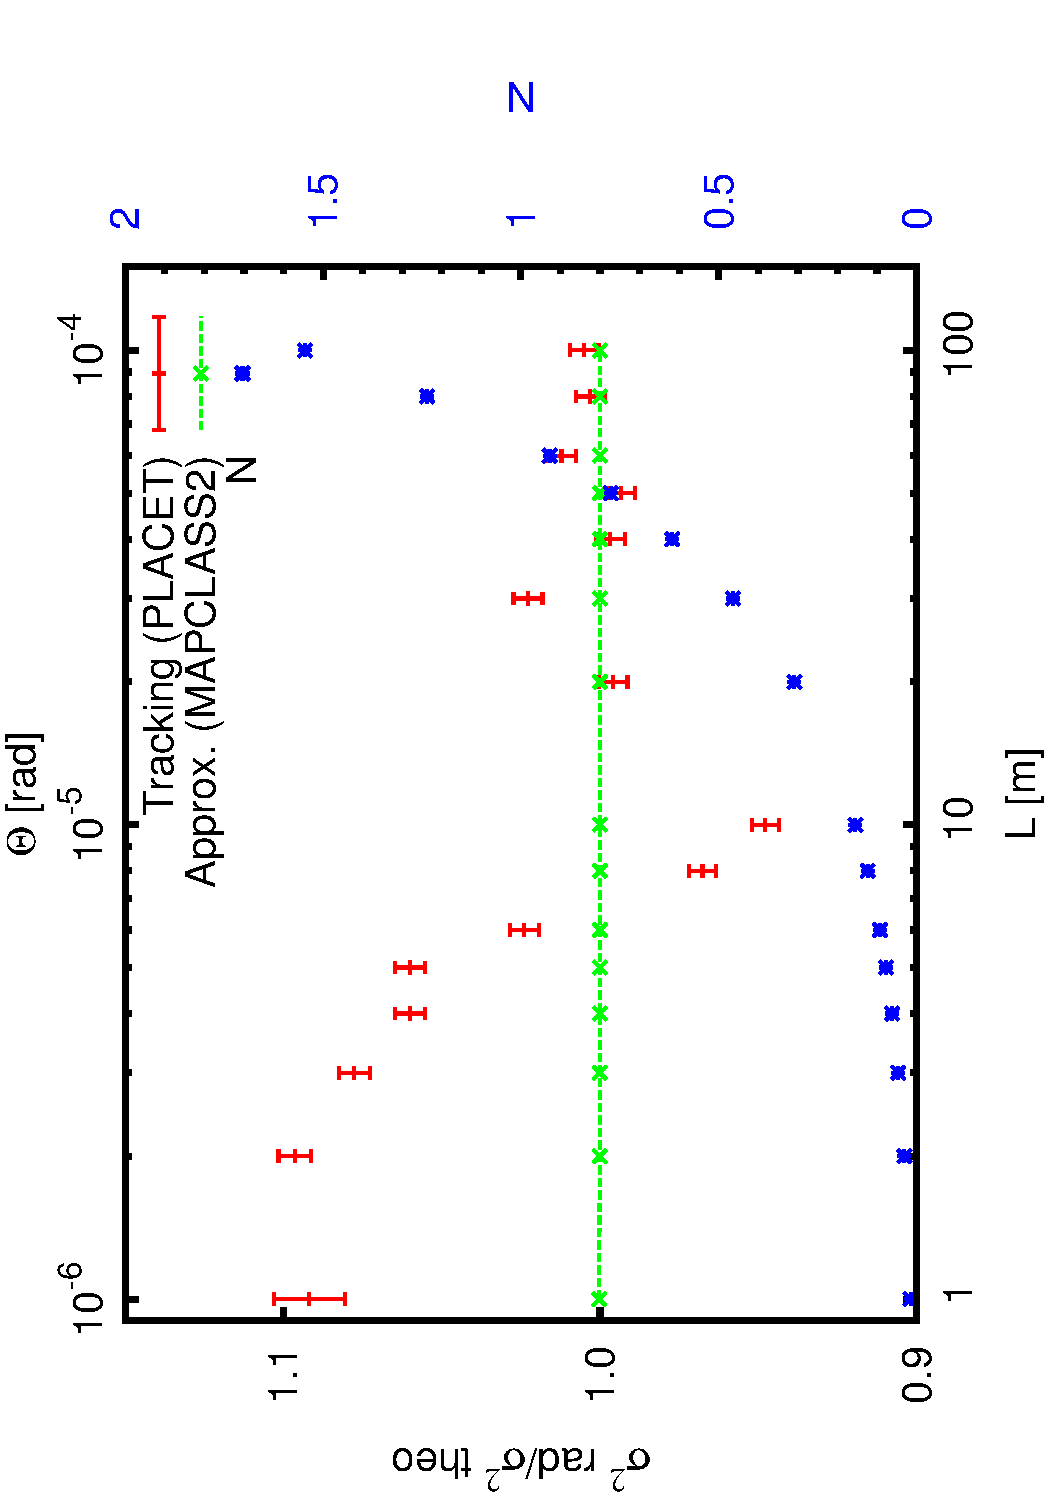
\includegraphics[scale=0.65,angle=-90]{./sigma_Bfix5e-3T.pdf} \caption{Result from tracking, theoretical calculation with the mean number of photons emitted by particle superimposed. Magnetic field is fixed at $5\times 10^{-3}$ T and $E=1500$ TeV.}\label{figPhotons}
\end{figure}
